\documentclass[tikz]{standalone}
\usepackage{framed}
\usepackage{amsmath} 
\usepackage{amsfonts}
\usepackage{xcolor}

\usetikzlibrary{decorations.pathmorphing}
\usetikzlibrary{arrows}

\begin{document}
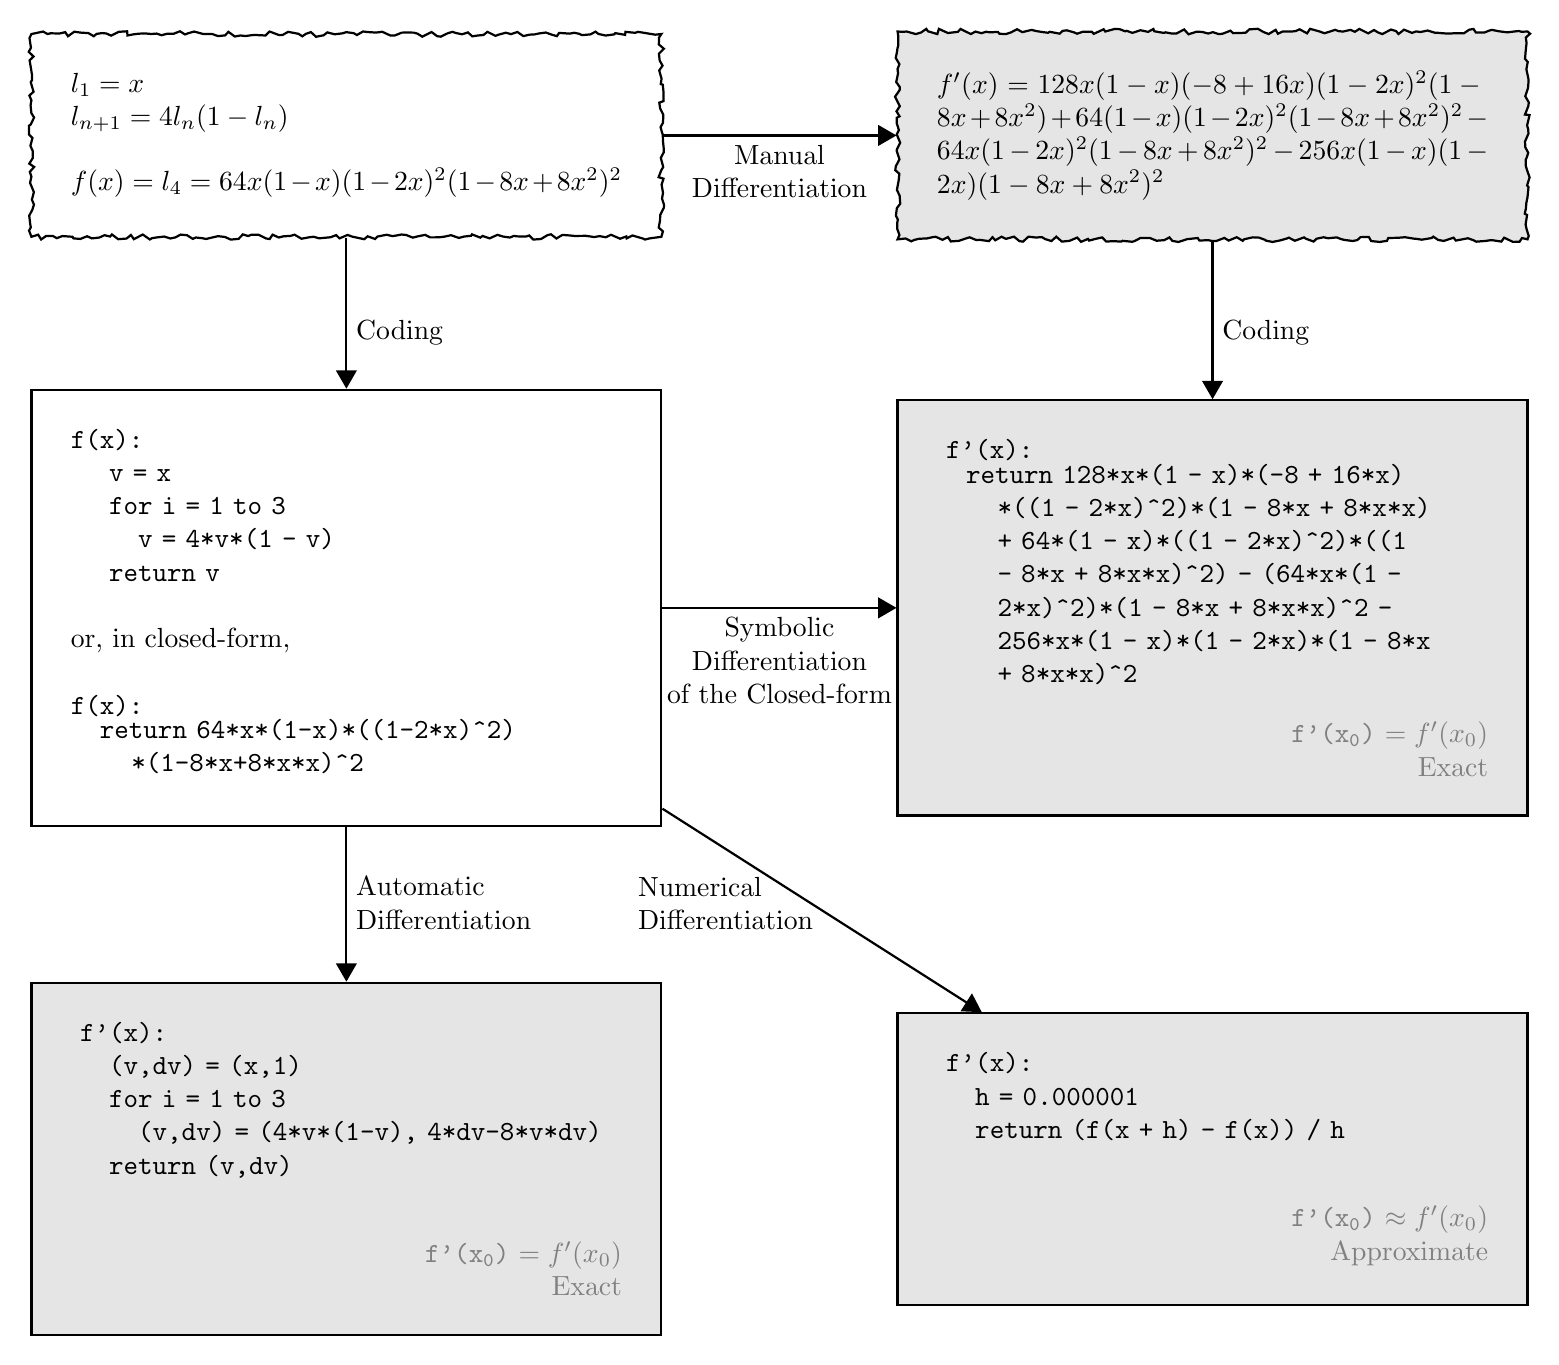
\begin{tikzpicture}[
	pencildraw/.style={
		decorate, 
		decoration={random steps,segment length=2pt,amplitude=1pt}
	}]
	%\draw[help lines] (0,0) grid (20,10);
	\tikzstyle{paperbox} = [pencildraw,draw,thick,fill=white,text width=7cm,inner sep=5mm]
	\tikzstyle{codebox} = [draw,thick,text width=7cm,inner sep=5mm]
	\tikzstyle{edge} = [->,>=triangle 60,thick]
	
    	\node[paperbox] (a) at (-5.5,-12.5) {
    	$l_1=x$\\
    	$l_{n+1}=4l_n(1-l_n)$\\
    	\vspace{4mm}
    	$f(x)=l_4=64x(1 - x)(1 - 2 x)^2 (1 - 8 x + 8 x^2)^2$
    	};
    	\node[paperbox,fill=gray!20] (b) at (5.5,-12.5) {$f'(x)=128x(1 - x)(-8 + 16 x)(1 - 2 x)^2(1 - 8 x + 8 x^2) + 64 (1 - x)(1 - 2 x)^2  (1 - 8 x + 8 x^2)^2 - 64x(1 - 2 x)^2 (1 - 8 x + 8 x^2)^2 - 256x(1 - x)(1 - 2 x)(1 - 8 x + 8 x^2)^2$};
    	\node[codebox,fill=white] (c) at (-5.5,-18.5) {\texttt{\parbox{7cm}{
		f(x):\\
    		\hphantom{tt} v = x\\
     		\hphantom{tt} for i = 1 to 3\\
        	\hphantom{tttt} v = 4*v*(1 - v)\\
    		\hphantom{tt} return v\\
		\hphantom{t}\\
    		\textrm{or, in closed-form,}\\
    		\hphantom{t}\\
    		f(x):\\
    		\hphantom{tt}\parbox{6cm}{\hangindent=0.4cm \hangafter=1 return 64*x*(1-x)*((1-2*x)\^{}2)\\ *(1-8*x+8*x*x)\^{}2}\\
	}}};
    	\node[codebox,black,fill=gray!20] (d) at (5.5,-18.5) {\color{black}\texttt{\parbox{7cm}{\textbf{
    		f'(x):\\
		\hphantom{tt}\parbox{6cm}{\hangindent=0.4cm \hangafter=1 return 128*x*(1 - x)*(-8 + 16*x)\\ *((1 - 2*x)\^{}2)*(1 - 8*x + 8*x*x)\\+ 64*(1 - x)*((1 - 2*x)\^{}2)*((1 - 8*x + 8*x*x)\^{}2) - (64*x*(1 - 2*x)\^{}2)*(1 - 8*x + 8*x*x)\^{}2 - 256*x*(1 - x)*(1 - 2*x)*(1 - 8*x + 8*x*x)\^{}2}\\}
		\flushright \color{gray} f'($\mathtt{x_0}$) $= f'(x_0)$\\\textrm{Exact}
	}}};
    	\node[codebox,black,fill=gray!20] (e) at (-5.5,-25.5) {\color{black}\texttt{\parbox{7cm}{\textbf{
		f'(x):\\
    		\hphantom{tt} (v,dv) = (x,1)\\
    		\hphantom{tt} for i = 1 to 3\\
        	\hphantom{tttt} (v,dv) = (4*v*(1-v), 4*dv-8*v*dv)\\
    		\hphantom{tt} return (v,dv)\\}
    		\flushright \color{gray} f'($\mathtt{x_0}$) $= f'(x_0)$\\\textrm{Exact}
	}}};
    	\node[codebox,black,fill=gray!20] (f) at (5.5,-25.5) {\color{black}\texttt{\parbox{7cm}{\textbf{
    		f'(x):\\
        \hphantom{tt} h = 0.000001\\
		\hphantom{tt} return (f(x + h) - f(x)) / h\\}
		\flushright \color{gray} f'($\mathtt{x_0}$) $\approx f'(x_0)$\\\textrm{Approximate}
	}}};
	
	\draw (a) edge [edge] (b);
    	\node[align=center,below] at (0,-12.5) {Manual\\Differentiation};
	
	\draw (c) edge [edge] (d);
    	\node[align=center,below] at (0,-18.5) {Symbolic\\Differentiation\\of the Closed-form};
    	
	\draw (a) edge [edge] (c);
	\node[align=left,right] at (-5.5,-15) {Coding};
    	
	\draw (b) edge [edge] (d);
	\node[align=left,right] at (5.5,-15) {Coding};
    	
	\draw (c) edge [edge] (f);
	\node[align=left,left] at (0.55,-22.25) {Numerical\\Differentiation};
    	
    	\draw (c) edge [edge] (e);
    	\node[align=left,right] at (-5.5,-22.25) {Automatic\\Differentiation};
    	
\end{tikzpicture}
\end{document}
